\documentclass[12pt, unicode]{beamer}
\usepackage{luatexja}
\usepackage{xurl}
\usepackage{tikz}
\usetikzlibrary{
  intersections,
  calc,
  arrows.meta,
  angles,
  quotes,
  graphs,
  positioning
}
\usetheme{metropolis}
\usepackage[absolute,overlay]{textpos}

\title{AIの過去・現在・未来 \\ 機械カニバリズム}
\author{淡中 圏}
\date{}

\begin{document}

\frame{\titlepage}

\begin{frame}{概略}

今日は「AIが現在のビジネス状況に与えるインパクト」みたいな話ではなく、もっと壮大な「AIの過去・現在・未来」について語る。

流れとしては:

生成系のAIは単なるAIの発展ではなく、AGI(汎用人工知能)への大きな一歩である(\textbf{自由エネルギー原理})。

汎用人工知能への道筋は(また勘違いの可能性もあるけど)かなり描けるようになってきた(\textbf{千の脳理論})。

そして、「人間のように自分の目的を持つ人工知能」も夢ではなくなってきた(\textbf{シンギュラリティ})。

\end{frame}

\begin{frame}{AIの歴史の概略}

AIの歴史は「知能って何?」という問いの歴史。

その時代に人間が知能について考えていたことがAIに反映される。
同時に、AIの発展が人間の知能を問い直してきた。

大雑把な流れとしては

\begin{itemize}
\item 人文的観点:言語や論理を重視
\item 生物的観点:フィードバックによる調節機能を重視
\end{itemize}

の二つがずっとあり、前者から後者に重心が移動してきた。

\end{frame}

\begin{frame}{AGI}

AIの中でも「何でもできるAI」を「AGI(汎用AI)」と呼ぶ。

人のように考える機械を作るアプローチには二つあった

\begin{itemize}
\item 人のように何でもできる機械(強いAI、AGI)をいきなり作る
\item とりあえず一つの分野についてできる機械(弱いAI))を作ってみる
\end{itemize}

\end{frame}
\begin{frame}{弱いAI}

最初は人文的観点からAGIが目指されたが、すぐにそれがとても難しいことがわかった。
その後、弱いAI、さらには生物的観点によって作られた弱いAIへと主軸が移ってきた。

ChatGPTも言語に特化した弱いAIであり、まだAGIではない。

\end{frame}

\begin{frame}{シンギュラリティについて}

シンギュラリティという言葉は曖昧なので、それについて語るのは非常に難しいが、
問題を明確にして「人間のように自分で目的を持つ機械」ができるかどうかは語れる。

そしてそれは\textbf{作れる}。

しかしそれを作るかどうか、作るべきかどうかについては議論がある。

ジェフ・ホーキンスの議論を紹介して、それに付言したい。

\end{frame}

\begin{frame}{AIの今後}

\centering
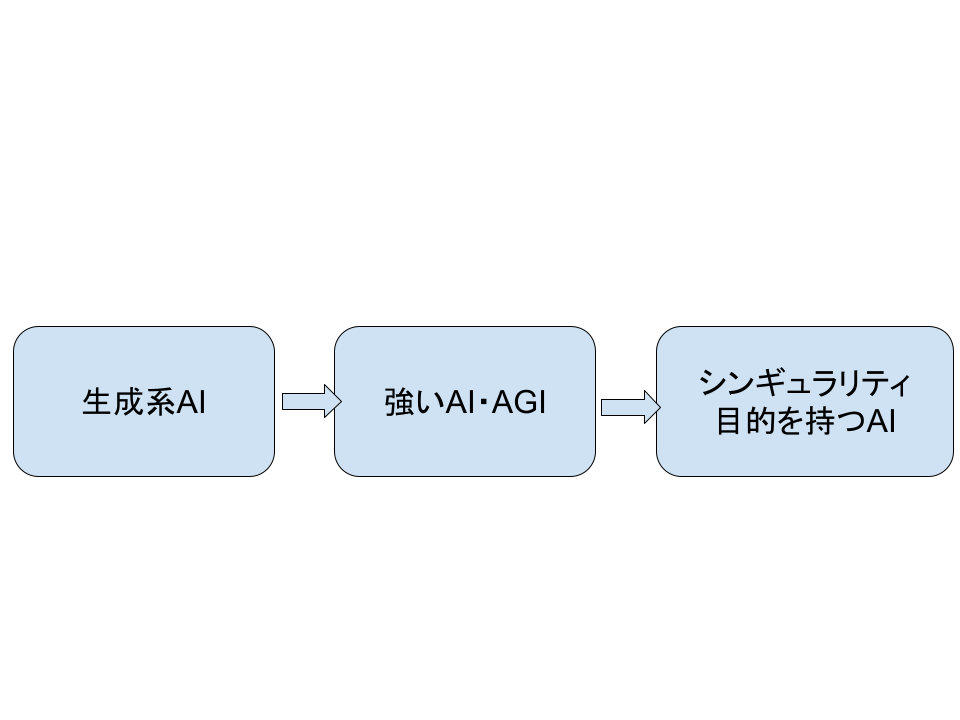
\includegraphics[keepaspectratio, scale=0.3]{ai_future.png}

\end{frame}

\begin{frame}{AI前史(人文側)}
 
人間の知能を人文側から「論理的推論能力」として見る観点はライプニッツやブールなど、以前からずっとあった。

またそれを自動化できないか、という発想もライプニッツからあった(計算機の発明、推論=計算という発想)

ここについて語ると長いので省略。

\end{frame}
\begin{frame}{AI前史(生物側)}

1930年代にノーバート・ウィーナーは、工学・生物学・社会学・計算機数学に共通する「情報」「コミュニケーション」「制御」
について研究する\textbf{サイバネティクス}という学際的分野を立ち上げた。

特に重要視された概念は\textbf{フィードバック}である。

脳とコンピュータとの関連もこの観点から研究された。

\end{frame}

\begin{frame}{AIの過去(人文側)}

初期のAI研究は、論理的な問題を解くことが中心だった。

研究者は画像認識や音声認識の問題もすぐに解けると思っていた。

しかし実世界の問題を解くのは非常に難しかった。

1980年台にエキスパートシステムなど一時的再流行も合ったものの、
「常識を学ばせることの難しさ」などにぶつかり、大きな成功は収めなかった。

\end{frame}

\begin{frame}{AIの過去(生物側)}

初期からパーセプトロンなど、ニューロンを模した学習システムは研究されたが、
すぐに限界が示された。

1980年代にはバック・プロパゲーションや勾配法など\textbf{深層学習}に必要な技術が出揃う。

しかし、あくまでこの時点では研究レベルにとどまっていた。

\end{frame}

\begin{frame}{現在(人文側)}

これらの技術の子孫はSAT/SMTや型検査や定理証明支援など、
今も大きな進歩をしているが、もはやAIとは呼ばれなくなっている。

\end{frame}

\begin{frame}{現在(生物側)}

GPU技術の発展により、2010年代から深層学習ブームが起こる。

画像認識などでいくつものブレイクスルーを起こし、ビジネス層にも強いインパクトを与えた。

しかし、ブーム初期の技術は実は1980年代に研究された技術の応用にすぎなかった。

それを覆したのが

\end{frame}

\begin{frame}{生成系AIの誕生}

\textbf{GAN(敵対的生成ネットワーク})による画像生成技術の発明である。

\end{frame}

\begin{frame}{生成系AIの衝撃}

GANは本物の人物写真そっくりの画像や、絵のスタイルを真似たり、絵のスタイルを混ぜたりといった画像生成で衝撃を与えた。

最初は、「面白いもののビジネスには繋がりにくい」という感じが多かったものの、拡散モデルやtransformerなど、さまざまな
発展があり、ついにChatGPTで大きなビジネス層へのインパクトをもたらした。

ここでは、生成系のAI技術が「知能とは何か」という問題にも大きな意味を持つことを語りたい。

\end{frame}

\begin{frame}{我々の心は常時予測をしている}

天然知能の驚くべき能力に「驚くことができる」というものがある。

「驚くことができる」ということは、実は我々が常時予測をしていることを意味している。

\end{frame}

\begin{frame}{脳の謎:内側から外側への情報の流れ}

脳の謎として、外側から内側への情報の流れと同じくらい、内側から外側への情報の流れがあることが知られていた。

以前は無視されがちだったこの情報の流れは、脳が「常時予測をし、それを実際の情報と比較し、修正をしている」というフィードバックループを描いていることの証拠ではないかと言われている。

\end{frame}

\begin{frame}{自由エネルギー原理}

このフィードバックループで\textbf{全て}を説明しようとするのがカール・フリストンの
\textbf{自由エネルギー原理(FEP)}という理論で現在一部でブームになっている。

この理論によれば、認知だけでなく、運動もホメオスタシスも全て「予測と現実のフィードバック(驚き最小の原則)」で実現されている。

注:何でも説明できちゃう怪しさもある……

\end{frame}

\begin{frame}

そういう意味で生成系AIの誕生は、「人間の脳のように考える機械」の誕生にとって大きな一歩である。

\end{frame}

\begin{frame}

それでは、最新のAI(例えばChatGPT)は\textbf{AGI(汎用人工知能)}なのか?

モデルはどこにあるのか?という議論で考えたい。

\end{frame}

\begin{frame}

FEPでは予測を作り出すために脳内に何らかの「モデル(予測をするための世界の模型)」があるとしている。
しかし、FEPではモデルの詳細についてあまり書いてないことが多い(気がする)。

人文的観点では「世界についての文章」がモデルになっていたが、生物的観点ではモデルがどのように作られているのかわかりにくい。

\end{frame}

\begin{frame}

深層学習では、ネットワーク内に「犬のモデル」「猫のモデル」のようなものができることがある。
しかし、それらはそれほどはっきりしたものではない。

もちろん生物の脳内でもそれははっきりしたものではないので、これは正しいとも言えるが、人間や他の生物が行なっているように
「操作可能な程度」にはこれらははっきりしたものである必要もある。

\end{frame}

\begin{frame}{環世界}
動物がどう世界とフィードバックし合っているかを考えるために便利な概念がユクスキュルの提唱した「環世界」である

ユクスキュルによると動物は世界全体ではなく、それぞれに特有な環世界から情報を得て生きている(例:マダニ)。

\vspace{-2\baselineskip}
\centering
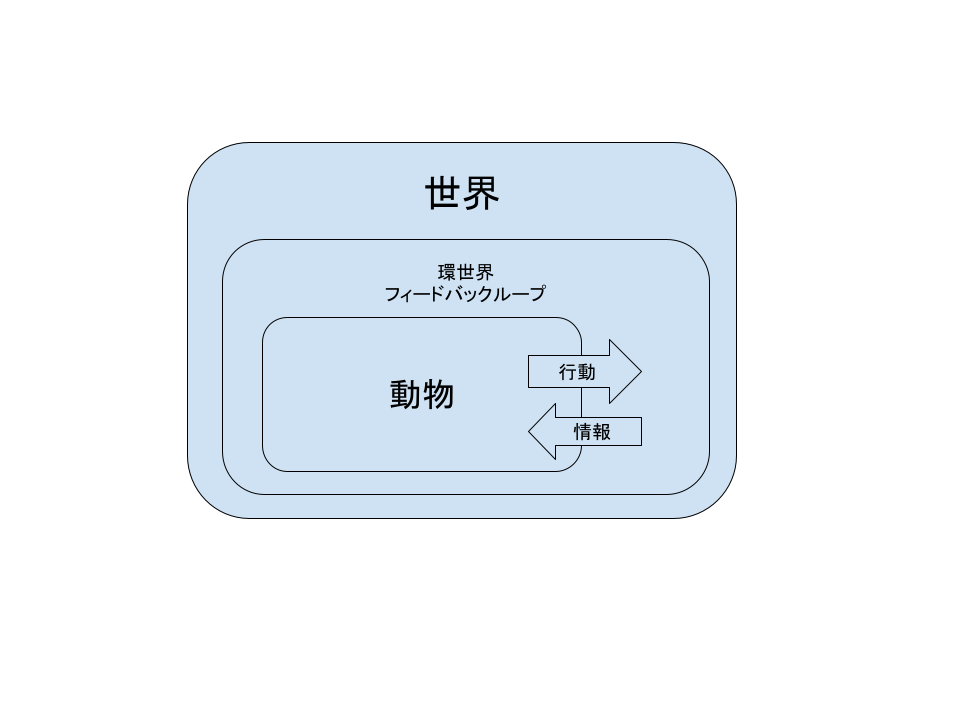
\includegraphics[keepaspectratio, scale=0.3]{umwelt.png}

\end{frame}
\begin{frame}

動物は環世界とフィードバックしあっている。

その結合度が高いと効率がいいが、環世界の変化に対応できなくなる。

その結合度が低ければ効率は悪くなるが、環世界の変化に対応できるようになる。

人間は環世界が変わっても対応ができる。ユクスキュルの言葉を借りれば、
人間の環世界は開かれている。

どうやって結合度を下げるのか。
プログラマにとっては日常的なことであるが、
結合度を低くする方法は、「モデル化による抽象化」である。

\end{frame}

\begin{frame}

密結合の状態と疎結合の状態にはトレードオフがある。
これは「人文⇔生物」の対立や
行動経済学における「オートモード⇔マニュアルモード」の対立と並行関係にある。

\vspace{-2\baselineskip}
\centering
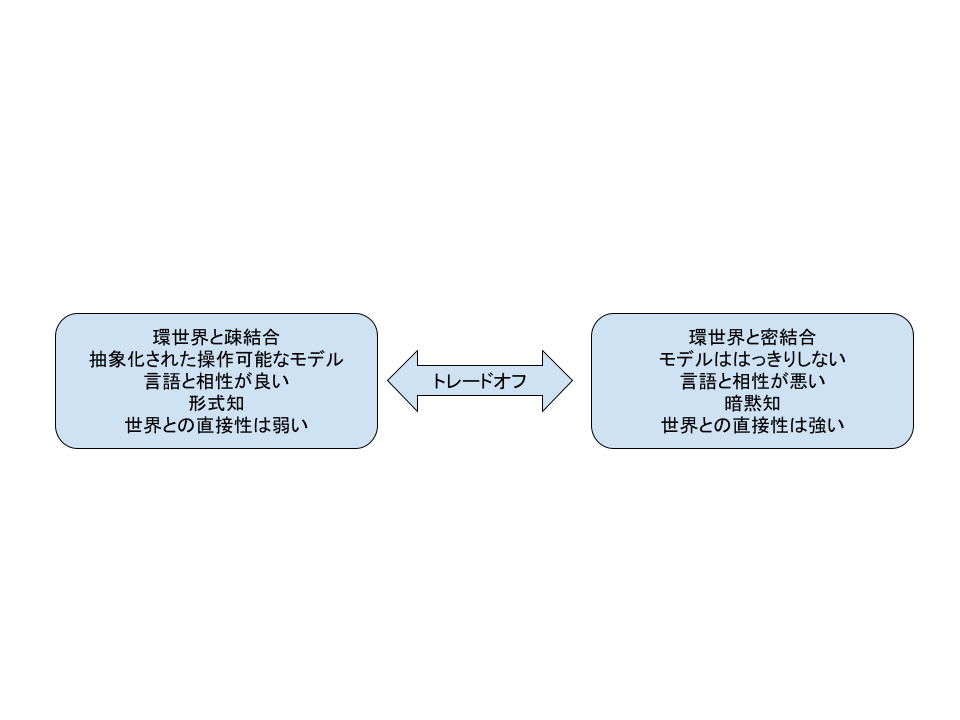
\includegraphics[keepaspectratio, scale=0.3]{open_umwelt.png}

\end{frame}

\begin{frame}

動物の脳に何らかの汎用的なモデル学習装置があると考えている人は多い。

そして現在ではそれは非言語的なものと考えられる(言葉を学習できなかった人や動物もある程度抽象化された思考をしている証拠がある)。

言語学者レイ・ジャッケンドフは『思考と意味の取扱いガイド』でそれは、
「脳内にあるイメージ(モデル)を連鎖的に発火させること」でなされている、としている。
そして言語は、その「脳内にあるイメージ」の「取っ手」として言語が優秀である、
として言語と思考の関係を説明する。

\end{frame}

\begin{frame}

現在のニューラルネットワークの研究では、
欲しいモデル(言語とか画像とか)に対してネットワークを設計する。
しかしそれでは、汎用的なモデル学習装置にはならない(抽象化ができない)。

また、リアルタイムの再学習にもあまり適していない(バッチで学習するしかなく、小さな学習ではせっかく学習したモデルが劣化しやすい)。

これらを解決する提案はすでに存在して、ジェフ・ホーキンスの「千の脳理論」である。

\end{frame}

\begin{frame}

ジェフ・ホーキンスは場所細胞と格子細胞という「空間を記憶するための細胞」が汎用のモデル学習装置として使えると指摘している(海馬の研究とも合致している)。

場所細胞と格子細胞は、「場所とそこにあるもの」「場所同士」の関係を学習してモデル化するための細胞である。

そしてこれは、空間的な情報に限らない、汎用のモデル学習装置になる(近い・遠いなどの空間的用語の汎用性。数学における幾何的道具の汎用性)。

\end{frame}

\begin{frame}
楽観的予想:

現在のさまざまな生成系AIの技術とジェフ・ホーキンスが考えているような汎用モデル学習装置を繋げれば、AGIができる可能性はある
(ジェフ・ホーキンスはAGIがその他のAIを駆逐すると、チップのアーキテクチャの歴史との類推で予測している)。

\end{frame}

\begin{frame}

それでは、「人間のように自分で目的を持つAI」についてジェフ・ホーキンスはどう考えているかというと……

\end{frame}

\begin{frame}

はっきりと「普通の作り方ではそういうAIにはならないし、そういう風に作る必要はない」と言っている。

\end{frame}

\begin{frame}

動物が目的を自分で持つのは動物が「ダーウィニズムで発生した」から。

ダーウィニズムで発生した動物は、「環境に繁殖のチャンスをいつも貪欲に探す」。

これが目的の元。

通常の作り方をしたニューラルネットワークにはこのような「貪欲さ」が育つ理由はない。

逆に言えば、AGIをこのような環境で育てれば、「自分で目的を持つAI」を作ることは可能!

\end{frame}

\begin{frame}

ただしそれを実際に作るかどうかは別問題。

ジェフ・ホーキンスは「そんなもの作る必要ないんじゃないか」とはっきり言っている。
そして自分で目的を持たないAGIも十分「知能がある」と考えて良い、としている。

ジェフ・ホーキンスにとってAIはあくまで道具。なので電源を切っても殺人にはならない(AIには目的を持たないので、死の恐怖もない)。

\end{frame}

\begin{frame}

でも、それは人間とはかなり違う「知能」だ。

この「知能」は

\begin{itemize}
\item こちらが呼びかけたりタスクを振らないと何もしない
\item 独り言も言わない
\end{itemize}

このような存在は、道具にはなるが「友達」にはなれない気がする。

\end{frame}

\begin{frame}{個人的見解}

作るべきかどうかはともかく、そのうち誰かが作ってしまう気がする。

そのような「自分で目的を持つAI」ができたらどうなるのか、の予測はほぼ無理だと考えている。

\end{frame}

\begin{frame}

とりあえず、しばらくはAGIができても、「目的を作る」という仕事は人類に残される。

なので、「目的を作る」ことに注力する必要がある。

\end{frame}

\begin{frame}{機械カニバリズム}

「自分で目的を持つAI」が誕生するまでは、AIはかなり人間と違う存在であり続ける(上位互換ではなく)。

その間の方針として、「機械カニバリズム(機械という他者を鏡として、人間とは何かを考え直し洗練させる)」が有効だと考えられる。

例えば将棋では、AIの「人間とはそもそも根本から違う」戦法を学ぶことで、人間の棋力がどんどん上がっているという現象が観測されている。

人文的AIの子孫である技術も、さまざまな点でそのような使われ方をしている。

\end{frame}

\begin{frame}

短期的にはさまざまな職種に大きなダメージがある(どんな職種にダメージがあるかは予測が難しい)。

長期的には「自分で目的を持つAI」まではとりあえず人類の仕事は消えない。

それまでは、「機械に得意なことは機械にやらせる。それなら人間がやることは何か?」という考えでやっていくしかない。

\end{frame}

\begin{frame}{終わりの言葉}

自ら想像した者をコントロールできない。
これこそまさに神の特権なのだから。

トーマス・パヴェル『エル・マハディ』

\end{frame}


\end{document}
